\documentclass[11pt,aspectratio=169]{beamer}
\usepackage[T1]{fontenc}
\usepackage[utf8]{inputenc}
\usepackage[english]{babel}
\usepackage{mathpazo}
\usefonttheme{serif}
\usepackage{amsmath,amssymb,booktabs,array,graphicx,microtype}
\usepackage{adjustbox}
\usepackage{tikz}
\usetikzlibrary{arrows.meta,calc,positioning,decorations.pathreplacing,patterns,fit,backgrounds}
\usepackage{animate}

% Figures and animations come from the idea folder; the TikZ figures in tikz/ are copies
% of those of the note.
\newcommand{\figdir}{../../../ideas/group-identification/figures}
\graphicspath{{../../../ideas/group-identification/figures/}}

% Colours of the note: i, j and a third flight; neutrals for text, grids and fills.
\definecolor{blueI}{HTML}{2A78D6}
\definecolor{orangeJ}{HTML}{EB6834}
\definecolor{aqua}{HTML}{1BAF7A}
\definecolor{ink}{HTML}{0B0B0B}
\definecolor{ink2}{HTML}{52514E}
\definecolor{muted}{HTML}{9A9893}
\definecolor{light}{HTML}{E6E5E1}
\definecolor{steel}{RGB}{74,96,121}
\definecolor{steellight}{RGB}{192,206,220}

\tikzset{
  >={Stealth[length=1.8mm]},
  every picture/.style={line cap=round, line join=round},
  track i/.style={blueI, line width=1.1pt},
  track j/.style={orangeJ, line width=1.1pt},
  track k/.style={aqua, line width=1.1pt},
  pt/.style={circle, inner sep=1.5pt, draw=ink, line width=0.4pt},
  pt i/.style={pt, fill=blueI},
  pt j/.style={pt, fill=orangeJ},
  pt k/.style={pt, fill=aqua},
  hollow j/.style={circle, inner sep=1.5pt, draw=orangeJ, fill=white, line width=0.9pt},
  lbl/.style={font=\footnotesize},
  note/.style={font=\footnotesize, text=ink2},
  tol/.style={draw=ink2, densely dashed, line width=0.5pt},
  flight/.style={circle, draw=ink, line width=0.6pt, minimum size=5.6mm, inner sep=0pt, font=\footnotesize, fill=white},
  inE1/.style={flight, fill=blueI, text=white},
  inE2/.style={flight, fill=orangeJ, text=white},
  edge/.style={ink, line width=1.2pt},
  bar/.style={draw=none, minimum height=3mm, inner sep=0pt},
  panel/.style={font=\small\bfseries, anchor=west},
}

\newcommand{\R}{\mathbb{R}}
\newcommand{\Z}{\mathbb{Z}}
\newcommand{\x}{\mathbf{x}}
\newcommand{\vh}{\hat{\mathbf{v}}}
\newcommand{\M}{\mathcal{M}}
\newcommand{\I}{\mathcal{I}}
\newcommand{\dep}{\mathrm{dep}}
\newcommand{\fin}{\mathrm{fin}}
\newcommand{\xc}{\mathrm{xc}}
\newcommand{\vis}{\mathrm{vis}}
\newcommand{\st}[1]{\textsf{#1}}
\newcommand{\ind}{\mathbf{1}}

% Theme: steel-blue title bar, white pages, as in the earlier decks.
\setbeamercolor{structure}{fg=steel}
\setbeamercolor{normal text}{fg=ink,bg=white}
\setbeamercolor{frametitle}{fg=white,bg=steel}
\setbeamercolor{alerted text}{fg=blueI}
\setbeamercolor{takeaway}{fg=steel,bg=steellight!30}
\setbeamercolor{defbox}{fg=ink,bg=steellight!28}
\setbeamersize{text margin left=7mm,text margin right=7mm}
\setbeamertemplate{navigation symbols}{}
\setbeamertemplate{itemize item}{\textcolor{steel}{\small$\bullet$}}
\setbeamertemplate{itemize subitem}{\textcolor{steel}{\textendash}}
\setbeamertemplate{itemize/enumerate body begin}{\setlength{\itemsep}{0.3em}}
\setbeamertemplate{frametitle}{%
  \nointerlineskip
  \begin{beamercolorbox}[wd=\paperwidth,ht=9mm,dp=3mm,center]{frametitle}
    \large\insertframetitle\strut
  \end{beamercolorbox}
  \begin{tikzpicture}[remember picture,overlay]
    \node[anchor=north east,text=white,inner sep=0pt,xshift=-2.3mm,yshift=-4.2mm]
      at(current page.north east){\small\insertframenumber};
  \end{tikzpicture}}
\setbeamertemplate{footline}{}

\newcommand{\source}[1]{\par\vspace{1mm}{\fontsize{7}{8.3}\selectfont\color{ink2}#1\par}}
\newcommand{\takeaway}[1]{\par\vfill
  \begin{beamercolorbox}[wd=\linewidth,sep=5pt]{takeaway}\small #1\end{beamercolorbox}}
% A definition: its name in bold, then the statement, on a pale band.
\newcommand{\defn}[2]{%
  \begin{beamercolorbox}[wd=\linewidth,sep=5pt]{defbox}\small\textcolor{steel}{\textbf{#1.}}\enspace #2\end{beamercolorbox}}
% A TikZ figure of the note, scaled to fit the given height and the line width.
\newcommand{\tikzfig}[2][0.8\textheight]{%
  \begin{center}\adjustbox{max width=\linewidth,max height=#1}{\input{tikz/#2}}\end{center}}
% An animation of the note; viewers without PDF JavaScript show its last frame.
\newcommand{\anim}[2]{\animategraphics[width=#1,controls={play,step,stop},loop,poster=last,
  timeline=\figdir/#2_frames.tln]{8}{\figdir/#2_frames}{}{}}
% The y axes of a three-panel figure set at .75\linewidth, one formula under each panel.
\newcommand{\yaxes}[3]{\makebox[.75\linewidth]{\small%
  \makebox[.25\linewidth]{$\displaystyle #1$}%
  \makebox[.25\linewidth]{$\displaystyle #2$}%
  \makebox[.25\linewidth]{$\displaystyle #3$}}}
% A full-page divider that opens one part of the talk.
\newcommand{\partframe}[2]{%
\begin{frame}[plain,noframenumbering]
\begin{tikzpicture}[remember picture,overlay]
 \fill[steel](current page.south west)rectangle(current page.north east);
 \node[text=white,align=center,text width=.82\paperwidth]at([yshift=4mm]current page.center)
   {{\Large\bfseries #1}\\[3mm]{\normalsize\color{steellight}#2}};
\end{tikzpicture}
\end{frame}}

\hypersetup{pdftitle={Group flight identification},pdfauthor={Matteo Di Sante},
  colorlinks=true,urlcolor=blueI,linkcolor=blueI}

\begin{document}

\begin{frame}[plain]
\begin{tikzpicture}[remember picture,overlay]
 \fill[steel](current page.south west)rectangle(current page.north east);
 \node[text=white,align=center,text width=.9\paperwidth]at(current page.center)
   {\LARGE\bfseries Identifying group flights in the FFVL archive};
\end{tikzpicture}
\end{frame}

\partframe{Part 1: the idea}{What the method does, on pictures}

\begin{frame}{The question}
\begin{beamercolorbox}[wd=\linewidth,sep=6pt,center]{takeaway}
\large For every flight and every instant: alone or in a group, and with whom?
\end{beamercolorbox}
\tikzfig[0.6\textheight]{requirements}
\par\small Pilots in a group need not take off from the same site, like $j$ and $k$.
\end{frame}

\begin{frame}{The method in six steps}
\tikzfig[0.8\textheight]{overview_idea}
\end{frame}

\begin{frame}{Two pilots on similar routes, 70--110~s apart}
\begin{columns}[c,onlytextwidth]
\column{.66\textwidth}
\anim{\linewidth}{contact_simple}
\column{.31\textwidth}
$j$ flies a route similar to that of $i$, here 70 to 110~s later: the
delay varies, we want it within $\delta$.
\par\bigskip
Same instant: here about 0.8~km apart, and it varies too.
\par\bigskip
Same place (within $\varepsilon_h$), with a delay (within $\delta$), seen from $i$ or from $j$:
\textbf{in contact}.
\end{columns}
\end{frame}

\begin{frame}{Configuration and group}
\tikzfig[0.58\textheight]{configuration_group}
\begin{columns}[T,onlytextwidth]
\column{.48\textwidth}
\small\textbf{Configuration}: gliders linked by contacts, with their links. A link more or
less: a new configuration.
\column{.48\textwidth}
\small\textbf{Group}: the same gliders, from a start to an end. It changes only when a glider
joins or leaves.
\end{columns}
\end{frame}

\begin{frame}{From configurations to episodes: an example day}
\begin{columns}[c,onlytextwidth]
\column{.64\textwidth}
\anim{\linewidth}{example_day}
\column{.33\textwidth}
\small
\textbf{Configuration} at $t$: gliders linked by chains of contacts, with their links.
\par\medskip
\textbf{Group}: the same members, from a start to an end. An arrival or a departure starts a
new one ($g_1,\dots,g_4$).
\par\medskip
\textbf{Episode}: a chain of groups, each group starting the instant the previous group ends and
sharing a member with it: $g_1\to g_2\to g_3$ is E1.\\ $g_4$ starts 50~min after $g_3$ ends: a new
episode, E2.
\end{columns}
\end{frame}

\partframe{Part 2: quantitative overview}{The same steps, with formulas}

\begin{frame}{Start at the departure}
\tikzfig[0.28\textheight]{local}
\defn{Departure}{
\[
  k^\dep_i=\min\bigl\{k:\ \|\x_i(k)-\x_i(k^0_i)\|>R_\dep\bigr\},\qquad R_\dep=3~\text{km}.
\]
Before it: local phase \st{L}.}
\defn{Evaluation instants}{
\[
  T^\dep_i=\bigl\{t\in\Delta\Z:\ k^\dep_i\le t\le k^\fin_i,\ \text{$i$ has a position at $t$}\bigr\},
  \qquad \Delta=5~\text{s}.
\]}
\end{frame}

\begin{frame}{Correspondence: the same place at two instants}
\defn{Correspondence}{One clock (UTC) for all flights: $i$ at instant $t$, $j$ at instant
$t'=t+l$, with $l$ the delay:
\[
  (t,t')\in\M_{ij}\iff |t'-t|\le\delta,\ \ \|\x_i(t)-\x_j(t')\|<\varepsilon_h,\ \
  |z_i(t)-z_j(t')|<\varepsilon_z,\ \ D_{ij}(t,t')=1
\]
$D_{ij}$ is the heading condition (next slide).}
\begin{columns}[c,onlytextwidth]
\column{.70\textwidth}
\tikzfig[0.45\textheight]{correspondence}
\column{.26\textwidth}
$\delta=2$~min\par
$\varepsilon_h=500$~m\par
$\varepsilon_z=300$~m
\end{columns}
\end{frame}

\begin{frame}{Heading condition: ruling out chance crossings}
Pilots who cross on different routes pass the distance and delay tests by chance.
A group flies the same way.
\tikzfig[0.30\textheight]{heading}
\defn{Heading condition}{
\[
  D_{ij}(t,t')=\begin{cases}
    \ind\bigl[\vh_i(t)\cdot\vh_j(t')>\cos\theta_{\max}\bigr] & \text{if both pilots glide},\\
    1 & \text{otherwise,}
  \end{cases}\qquad \theta_{\max}=45^\circ.
\]}
\smallskip
{\small Phases (Vilpellet) exist only on 1~Hz flights. The other flights are grouped all the same,
without this condition: distance, height and delay alone.\par}
\end{frame}

\begin{frame}{Contact: what $i$ sees, what $j$ sees}
\begin{columns}[c,onlytextwidth]
\column{.63\textwidth}
\anim{\linewidth}{views}
\column{.34\textwidth}
\defn{Contact}{\small
\[
  \begin{aligned}
    m_{ij}(t)&=\ind\bigl[\exists\,t':(t,t')\in\M_{ij}\bigr]\\
    m_{ji}(t)&=\ind\bigl[\exists\,t':(t',t)\in\M_{ij}\bigr]\\
    a_{ij}&=m_{ij}\vee m_{ji}
  \end{aligned}
\]}
\par\medskip
\small
$j$ joins the route of $i$, 90~s behind, then leaves it.
\par\medskip
Start: $m_{ij}=1$, $m_{ji}=0$. End: the reverse.
\par\medskip
$m_{ij}\ne m_{ji}$ in general; the contact $a_{ij}=a_{ji}$ is symmetric.
\end{columns}
\end{frame}

\begin{frame}{Pair intervals: fill short gaps, drop short contacts}
\tikzfig[0.3\textheight]{pair_intervals}
\defn{Pair interval}{A run of $a_{ij}=1$, gaps $<\boldsymbol{g=120}$~\textbf{s} joined, lasting
$\ge\boldsymbol{\tau^*=38.1}$~\textbf{min}: $[t_{\rm on},t_{\rm off})$.}
\defn{Choosing $\tau^*$}{Not set by hand: we fix $q=10\%$, the share of kept intervals we accept
to be chance. The null model (pairs shifted in time) counts the chance intervals $C(\tau)$
among the $N(\tau)$ observed:
\[
  \tau^*=\min\Bigl\{\tau:\ \frac{C(\tau)}{N(\tau)}\le q\Bigr\}.
\]
Smaller $\tau^*$: more intervals, more of them chance. Larger $\tau^*$: fewer, cleaner.}
\end{frame}

\begin{frame}{Contact is not transitive: three ways to define groups}
\tikzfig[0.62\textheight]{transitivity}
\small (a) and (b): one picture of the whole day, without time. (c): one picture per instant; 8 is
in two groups, never at the same instant.
\end{frame}

\begin{frame}{Active graph: the configurations at one instant}
\defn{Active graph}{
\[
  G(t)=\bigl(V(t),E(t)\bigr),\qquad
  V(t)=\text{flights in the air at }t,\qquad
  E(t)=\bigl\{\{i,j\}:\ t\in[t_{\rm on},t_{\rm off})\bigr\}.
\]}
\tikzfig[0.4\textheight]{active_graph}
\defn{Configuration}{At $t$: a connected component of $G(t)$ with two or more flights, with its
edges.}
\end{frame}

\begin{frame}{Group: fixed members, changing configurations}
\tikzfig[0.42\textheight]{configurations}
\begin{columns}[T,onlytextwidth]
\column{.49\textwidth}
\defn{Group}{$g=\bigl(M_g,[t^{\rm start}_g,t^{\rm end}_g)\bigr)$: $M_g$ are the members of a
configuration of $G(t)$ at every $t$ of the interval, and the interval is maximal.}
\column{.49\textwidth}
\defn{Membership}{
\[
  \gamma_i(t)=\begin{cases}
    \st{L} & \text{before the departure},\\
    g & i\in M_g,\ t\in[t^{\rm start}_g,t^{\rm end}_g),\\
    \st{S} & \text{otherwise (solo).}
  \end{cases}
\]}
\end{columns}
\end{frame}

\begin{frame}{Episode: groups linked in time}
\tikzfig[0.4\textheight]{episodes}
\defn{Episode}{Link $g\to g'$: $g'$ starts the instant $g$ ends, and they share a member,
\[
  t^{\rm start}_{g'}=t^{\rm end}_g,\qquad M_g\cap M_{g'}\ne\emptyset .
\]
An episode: a connected component of the graph of these links. $g_1$ and $g_2$ have no link between
them, but both link to $g_3$: all three are in E1.}
\end{frame}

\begin{frame}{On the FFVL archive}
\begin{columns}[t,onlytextwidth]
\column{.24\textwidth}
\centering
{\Huge\textcolor{blueI}{21.7\%}}\par\smallskip
\small of paraglider flights fly in a group at some point\par
\column{.24\textwidth}
\centering
{\Huge\textcolor{orangeJ}{6.9\%}}\par\smallskip
\small of hang-glider flights\par
\column{.24\textwidth}
\centering
{\Huge\textcolor{steel}{17\,169}}\par\smallskip
\small episodes
\column{.24\textwidth}
\centering
{\Huge\textcolor{steel}{58 min}}\par\smallskip
\small median episode; 2 flights (median), up to 53
\end{columns}
\source{160\,637 flights; $\delta=2$~min, $\varepsilon_h=500$~m, $\varepsilon_z=300$~m, $g=120$~s,
$\tau^*=38.1$~min.}
\end{frame}



\begin{frame}{Episodes: how long, how many flights}
\begingroup\centering
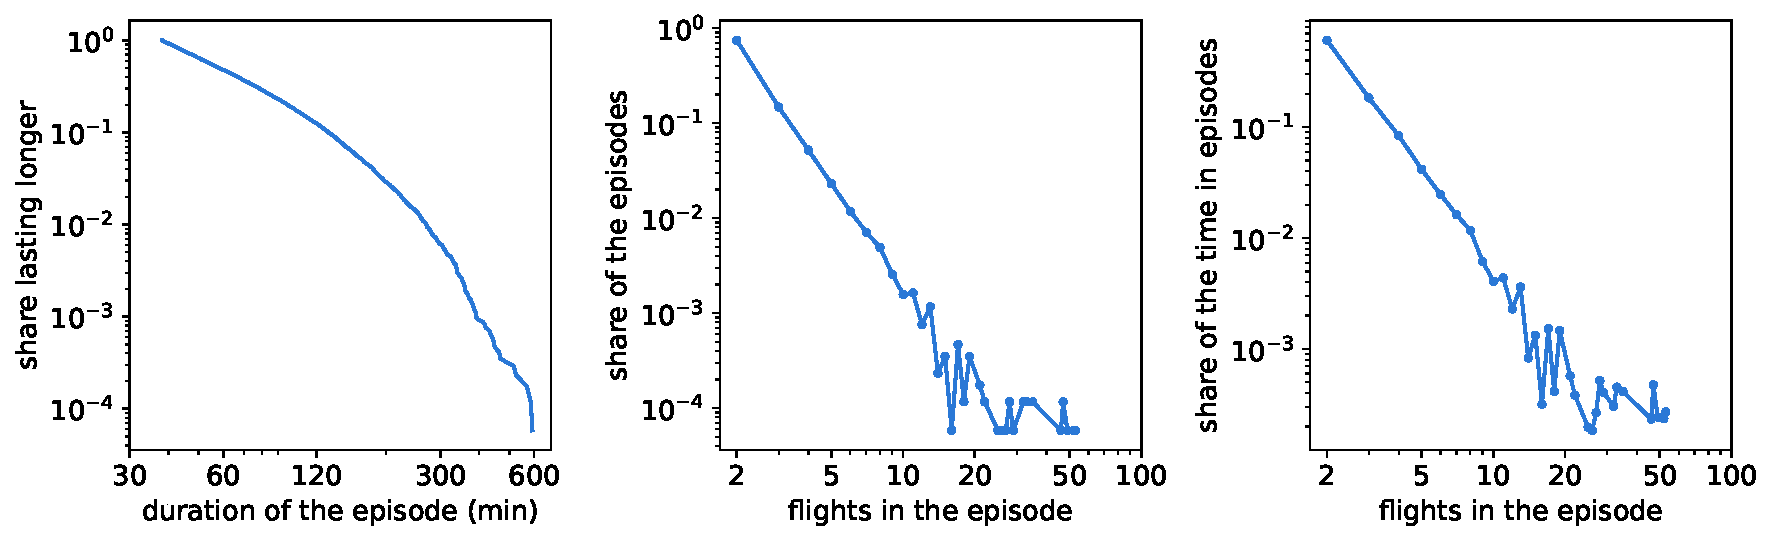
\includegraphics[width=.75\linewidth]{assessment_structure_episodes_q01.pdf}\par
\yaxes{y=\frac{\#\{E:\ D_E\ge d\}}{N}}{y=\frac{N_n}{N}}{y=T(n)=\frac{\sum_{E:\,n_E=n}D_E}{\sum_E D_E}}\par\endgroup
\source{Episode $E$: $D_E$ from the start of its first group to the end of its last, $n_E$ its distinct
flights. $N=17\,169$ episodes, $N_n$ of them with $n_E=n$. Whole archive, $\delta=2$~min, $q=0.1$.}
\par\smallskip\small $T(n)$: of every 100~s of episode time, summed over all episodes, on average
$100\,T(n)$~s are in episodes of $n$ flights; for $n=5$, 4.2~s.
\takeaway{The median episode lasts 58~min and 74\% are pairs. Weighted by time
the pairs drop to 61\%: large episodes last longer.}
\end{frame}

\begin{frame}{Groups: how long, how many pilots at once}
\begingroup\centering
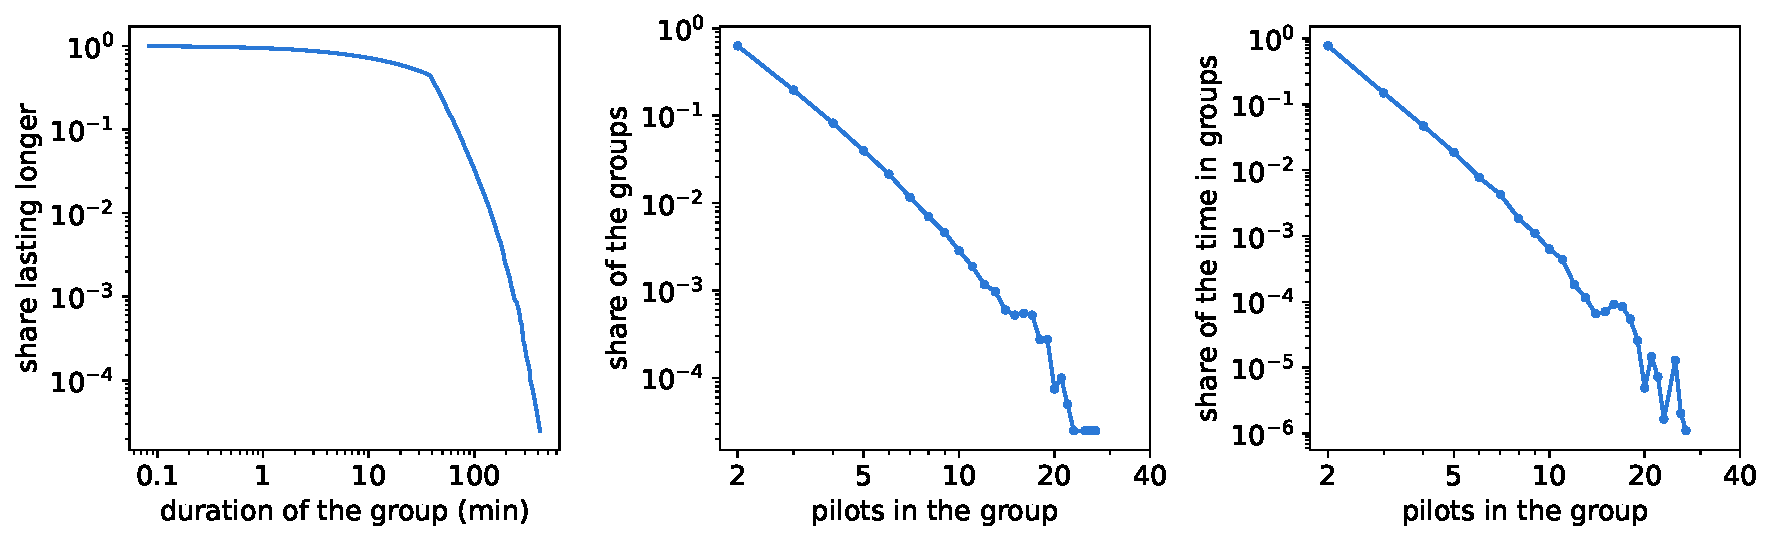
\includegraphics[width=.75\linewidth]{assessment_structure_groups_q01.pdf}\par
\yaxes{y=\frac{\#\{g:\ D_g\ge d\}}{N}}{y=\frac{N_n}{N}}{y=T(n)=\frac{\sum_{g:\,n_g=n}D_g}{\sum_g D_g}}\par\endgroup
\source{Group $g$: $D_g=t^{\rm end}_g-t^{\rm start}_g$, $n_g=|M_g|$ its pilots; each arrival or departure
starts a new group. $N=40\,051$ groups, $N_n$ of them with $n_g=n$. Whole archive, $\delta=2$~min,
$q=0.1$.}
\par\smallskip\small $T(n)$: of every 100~s of group time, summed over all groups, on average
$100\,T(n)$~s are in groups of $n$ pilots; for $n=5$, 1.9~s. A group counts its duration once,
not once per pilot.
\takeaway{Median group 30~min, 63\% are pairs. Weighted by time the pairs rise to
77\%: large groups change quickly.}
\end{frame}


\begin{frame}{Who follows whom: the delay}
\defn{Delay}{At $t$, the delay at which $j$ is closest to $i$ in 3D, $\mathbf X=(\x,z)$; over a
pair interval, the median:
\[
  l^*(t)=\arg\min_{l:\,(t,t+l)\in\M_{ij}}\|\mathbf X_i(t)-\mathbf X_j(t+l)\|,\qquad
  \ell_{\rm med}=\mathrm{median}\,l^*,\qquad \ell_{\rm med}>0:\ j\ \text{follows}\ i.
\]}
\begin{columns}[c,onlytextwidth]
\column{.64\textwidth}
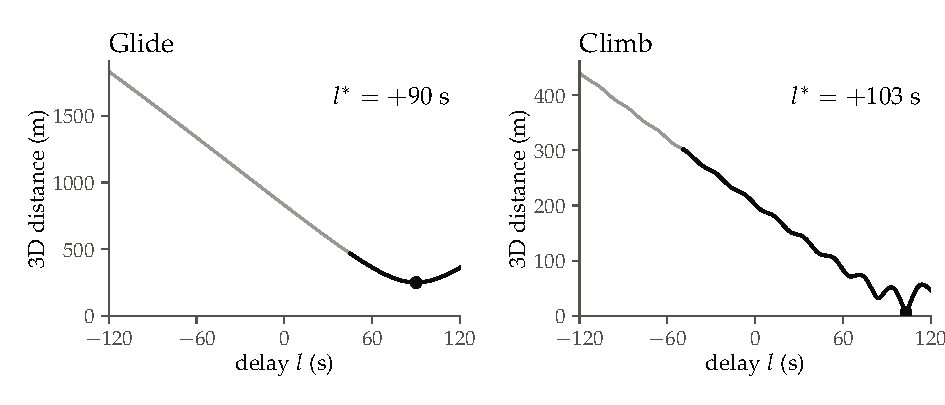
\includegraphics[width=\linewidth]{delay.pdf}
\column{.33\textwidth}
\small
\textbf{Glide}: one sharp minimum, where $j$ crosses the point of $i$.
\par\medskip
\textbf{Climb}: one dip per turn; the altitude picks the turn.
\par\medskip
\textbf{Search}: no climb, so nothing picks the turn: left out of $\ell_{\rm med}$.
\end{columns}
\source{Models: glide, $j$ 90~s behind and 250~m to the side; climb, $j$ 200~m lower, both at 2~m/s,
circles of 25~m, one turn per 20~s; $\delta=2$~min.}
\end{frame}


\end{document}
